\section{Medien}

\subsection{Bilder}

\begin{figure}[H]
	\centering
	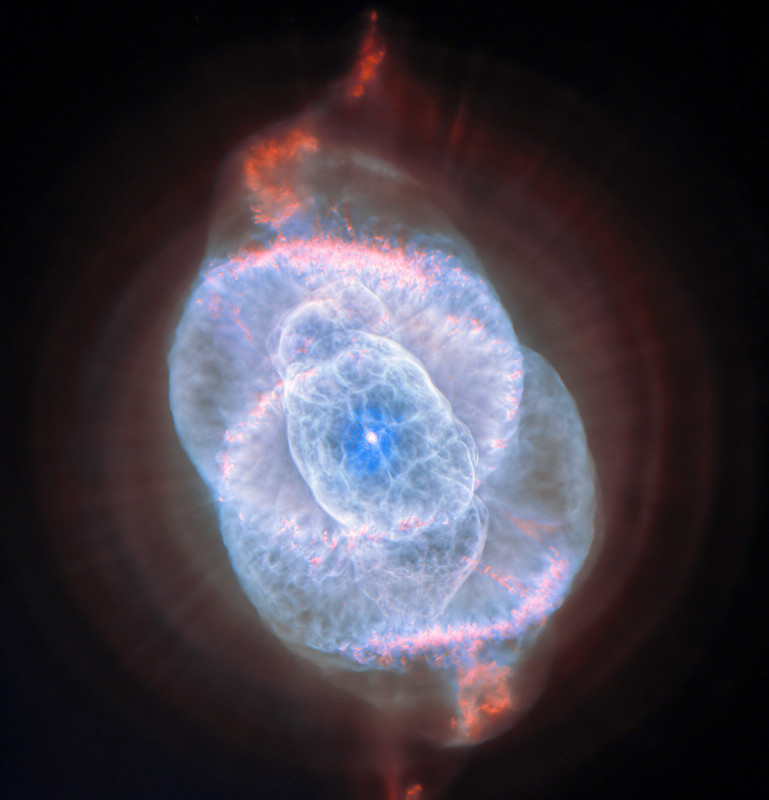
\includegraphics[width=0.4\linewidth]{images/nasa_hubble_cats_eye_nebula.jpg}

	\caption{Bild \texttt{[H]} welches zu Groß ist für die aktuelle Seite aber den folgenden Inhalt blockiert im Gegesatz zum Standardverhalten welcher diesen schon auf der vorherigen Seite platzieren würde}
	\label{fig:imageFloat}
\end{figure}

Referenziere Abbildung~\ref{fig:imageFloat} im Text.

\begin{figure}[ht]
	\centering
	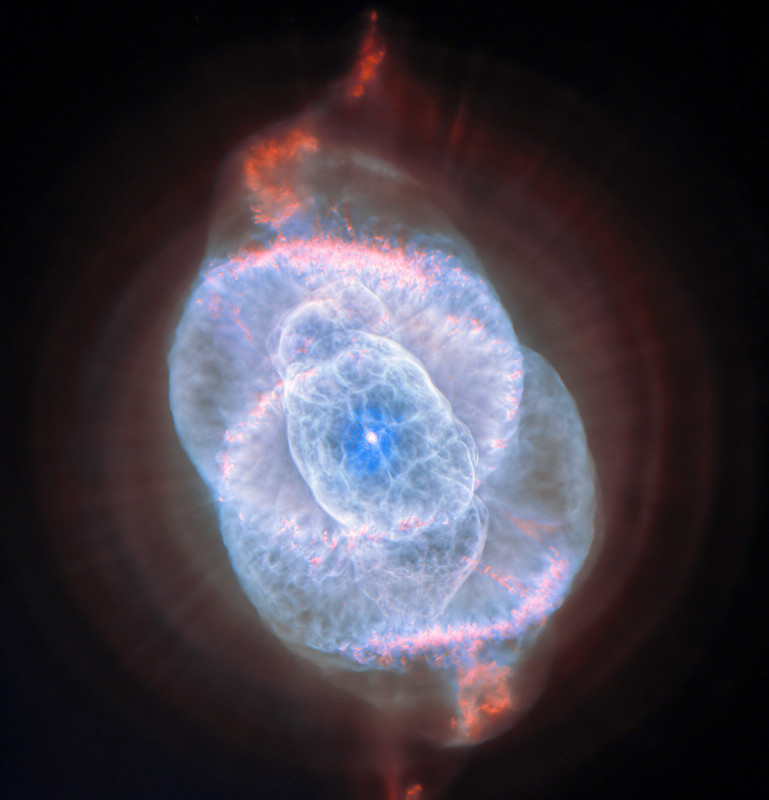
\includegraphics[width=0.5\linewidth]{images/nasa_hubble_cats_eye_nebula.jpg}

	\caption{Bild \texttt{[ht]}}
	\label{fig:imageNormal}
\end{figure}

\begin{figure}[ht]
	\centering
	\begin{subfigure}[b]{0.48\textwidth}
		\centering
		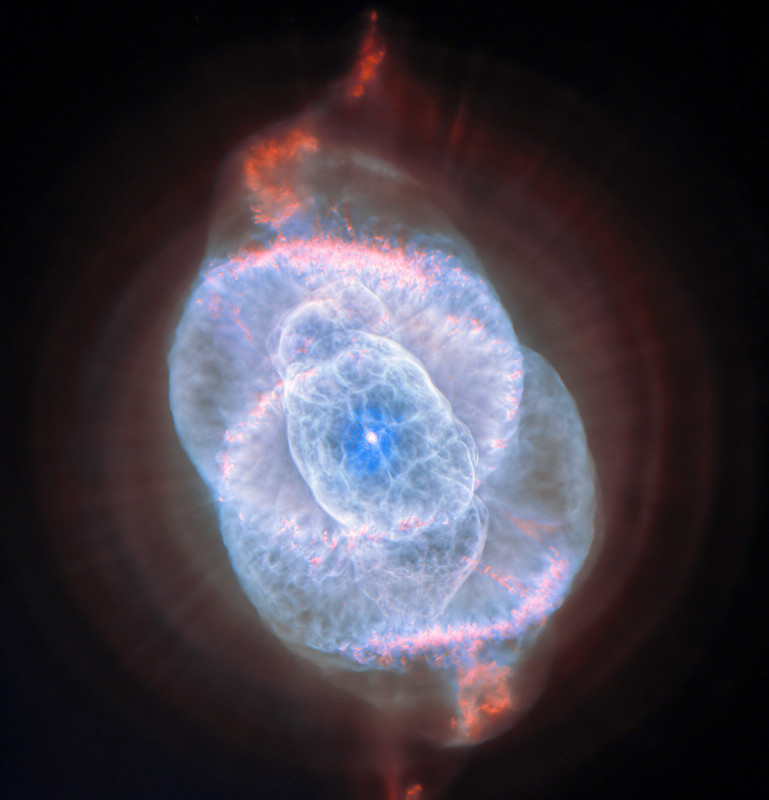
\includegraphics[width=\linewidth]{images/nasa_hubble_cats_eye_nebula.jpg}

		\caption{Linkes Bild}
		\label{fig:imageSubLeft}
	\end{subfigure}
	\hfill
	\begin{subfigure}[b]{0.48\textwidth}
		\centering
		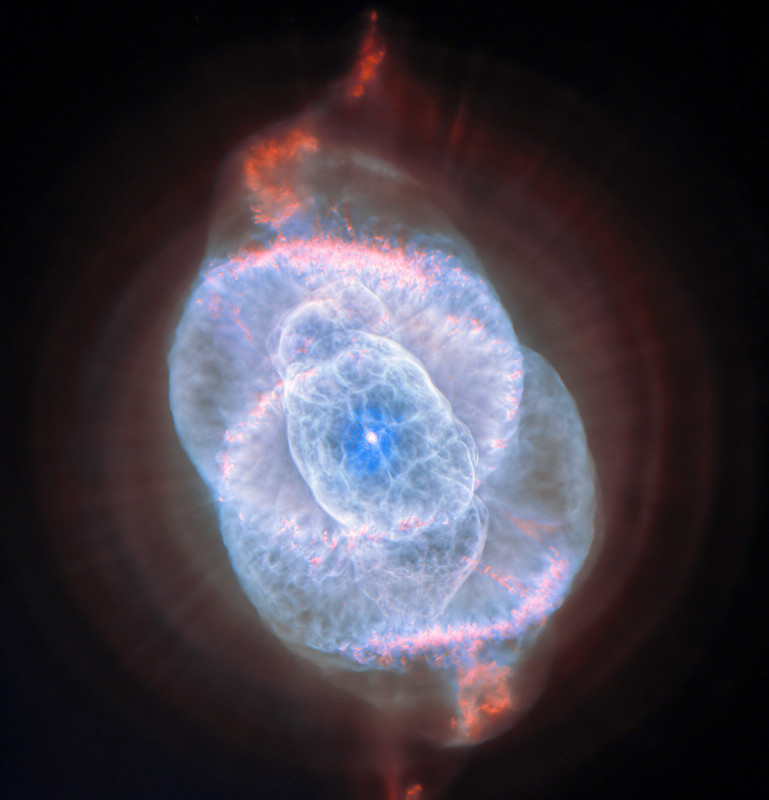
\includegraphics[width=\linewidth]{images/nasa_hubble_cats_eye_nebula.jpg}

		\caption{Rechtes Bild}
		\label{fig:imageSubRight}
	\end{subfigure}

	\caption{Mehrere Bilder}
	\label{fig:multipleImages}
\end{figure}

\begin{figure}[H]
	\centering
	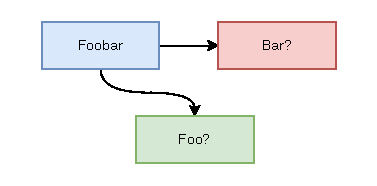
\includegraphics[width=0.4\linewidth]{images/graph.drawio.pdf}

	\caption{Vektorgrafik Bild \texttt{(.pdf)}}
	\label{fig:imageVector}
\end{figure}
